\section{概要}

\index{Framework}

\begin{figure}[t]
\begin{center}
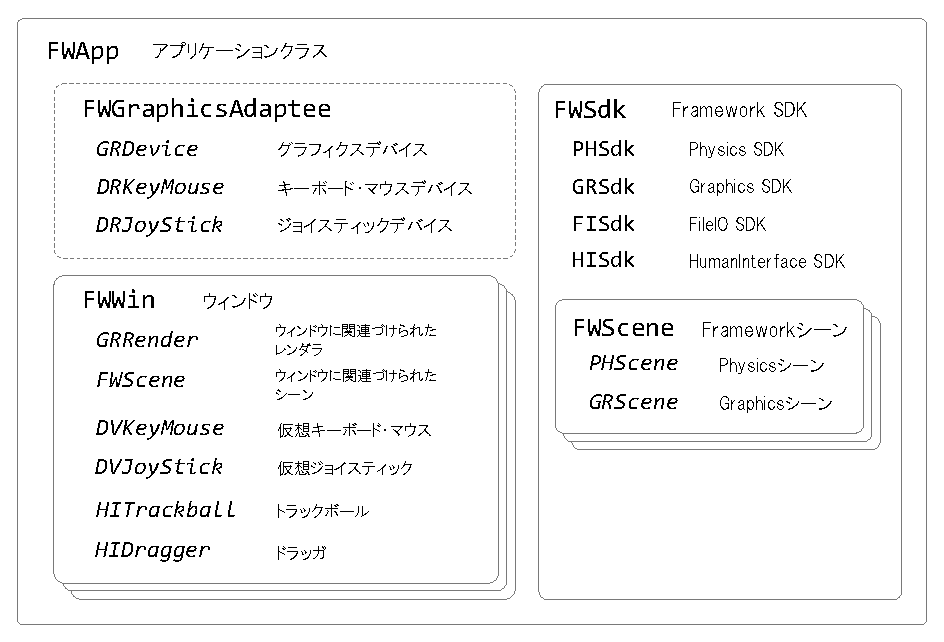
\includegraphics[width=.7\hsize]{fig/framework.eps}
\end{center}
\caption{Framework data structure}
\label{fig_framework}
\end{figure}


Frameworkはモジュール間の連携を促進してアプリケーションの作成を支援するためのモジュールです.

Frameworkモジュールのデータ構造をFig.\,\ref{fig_framework}に示します.
\KLUDGE 最上位にはアプリケーションクラス\texttt{FWApp}があります.
\KLUDGE ユーザは\texttt{FWApp}を継承することで独自のアプリケーションを作成します.
\texttt{FWApp}その中にトップレベルウィンドウ(\texttt{FWWin})の配列,Framework SDK (\texttt{FWSdk}),
\KLUDGE およびウィンドウマネジャ(\texttt{FWGraphicsAdaptee})を持ちます.

\texttt{FWWin}はトップレベルウィンドウで,そのウィンドウに対応する入力デバイスやビューポート情報を保持するレンダラ,
\KLUDGE そのウィンドウと関連付けられたシーンへの参照などを持ちます.
\KLUDGE また,図中では省略されていますがサブウィンドウやGUIコントロールを持つこともできます.

\texttt{FWSdk}の役割は周辺モジュールの機能統合です.
\KLUDGE その中に周辺モジュールのSDKクラスやFrameworkシーン(\texttt{FWScene})の配列を持ちます.

\KLUDGE ウィンドウマネジャは処理系に依存するデバイスの初期化やイベントハンドリングを行います.
\KLUDGE ウィンドウマネジャはインタフェースを公開していませんのでユーザはその存在を陽に意識する必要はありません.
\KLUDGE 図ではデータ構造の説明のためにあえて記載しています.

\KLUDGE 以下では個々の構成要素について説明していきます.


\section{Framework SDK}

\index{FWSdk}
FrameworkモジュールのすべてのオブジェクトはSDKクラス\texttt{FWSdk}によって管理されます.
\texttt{FWSdk}クラスは,プログラムの実行を通してただ1つのオブジェクトが存在するシングルトンクラスです.
\texttt{FWSdk}オブジェクトを作成するには以下のようにします.
\begin{sourcecode}
FWSdkIf* fwSdk = FWSdkIf::CreateSdk();
\end{sourcecode}
\KLUDGE 通常この操作はプログラムの初期化時に一度だけ実行します.
\texttt{FWSdk}を作成すると,同時に\texttt{PHSdk},\texttt{GRSdk},\texttt{FISdk},\texttt{HISdk}も作成されます.
\KLUDGE したがってこれらをユーザが手動で作成する必要はありません.
\KLUDGE 各モジュールの機能にアクセスするには以下の関数によりSDKを取得します.

\noindent
\begin{tabular}{p{1.0\hsize}}
\\
\texttt{FWSdkIf}				\\ \midrule
\texttt{PHSdkIf* GetPHSdk()}	\\
Physics SDKを取得する.			\\
\\
\texttt{GRSdkIf* GetGRSdk()}	\\
Graphics SDKを取得する.		\\
\\
\texttt{FISdkIf* GetFISdk()}	\\
FileIO SDKを取得する.			\\
\\
\texttt{HISdkIf* GetHISdk()}	\\
HumanInterface SDKを取得する.	\\
\\
\end{tabular}

\section{Framework シーン}

\begin{figure}[t]
\begin{center}
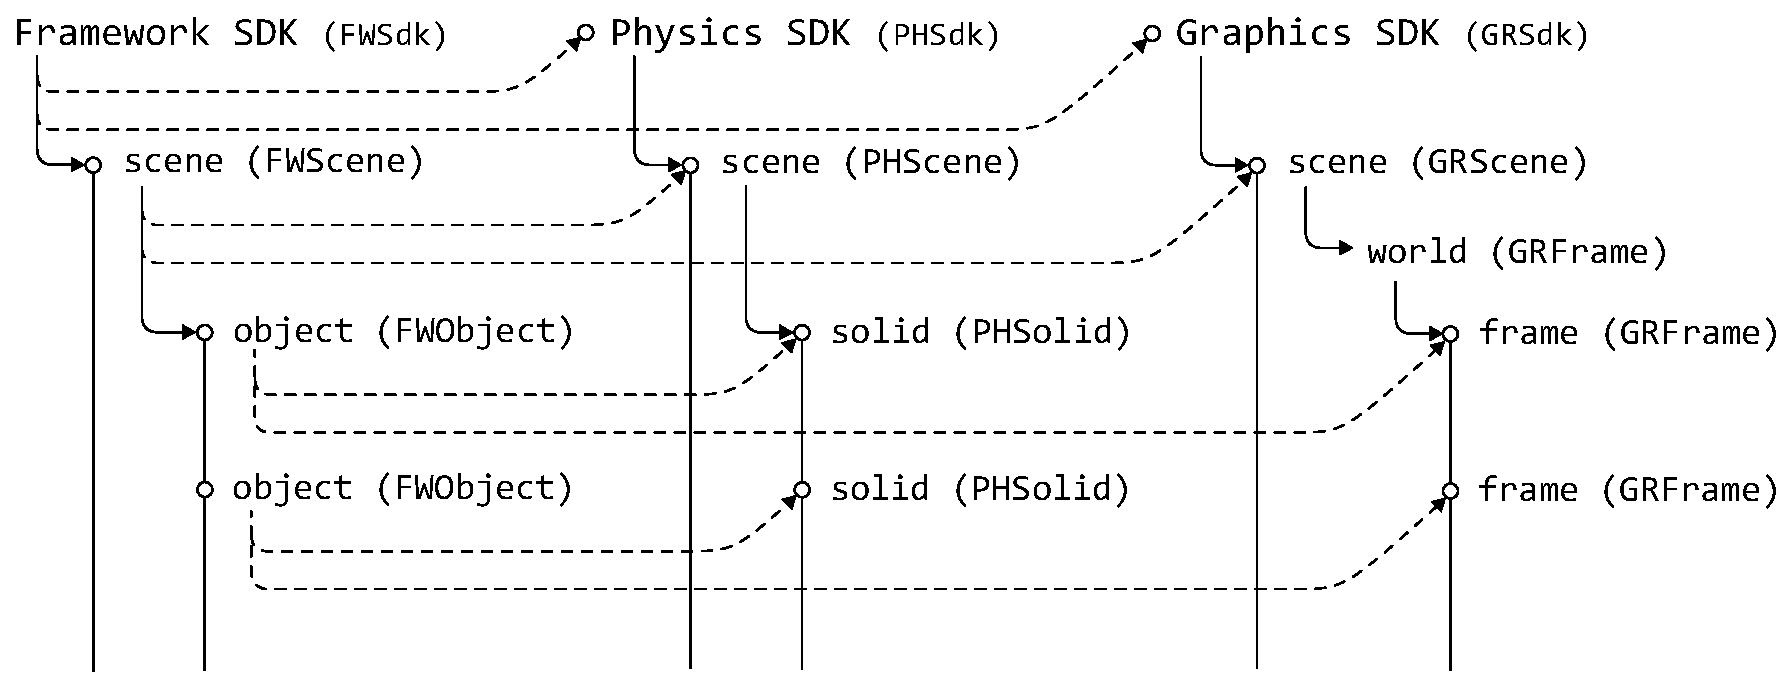
\includegraphics[width=.9\hsize]{fig/fwscene.eps}
\end{center}
\caption{Data structure of Framework, Physics and Graphics modules}
\label{fig_fwscene}
\end{figure}

\index{FWScene}
\index{FWObject}
Frameworkモジュールの主な機能の1つにPhysicsシーンとGraphicsシーンの同期があります.
Fig.\,\ref{fig_fwscene}に3つのモジュールのSDKとシーンの関係を示します.
\texttt{FWSdk}は任意の数のシーン(\texttt{FWScene}クラス)を保持します.
\KLUDGE また,シーンは任意の数のオブジェクト(\texttt{FWObject}クラス)を保持します.
Fig.\,\ref{fig_fwscene}に示すように,
\KLUDGE オブジェクトはPhysicsモジュールの剛体とGraphicsモジュールのトップフレームを一対一に対応づけます.
\KLUDGE ここでトップフレームとはワールドフレームの直下にあるフレームのことです.
\KLUDGE 物理シミュレーションにより計算される剛体の運動をフレームの座標変換に反映させることで,
\KLUDGE シミュレーションの様子をGraphicsモジュールの機能を利用して可視化することができるようになります.

\KLUDGE シーン作成に関する\texttt{FWSdk}の関数を以下に示します.

\noindent
\begin{tabular}{p{1.0\hsize}}
\\
\texttt{HITrackballIf}														\\ \midrule
\texttt{FWSceneIf* CreateScene(const PHSceneDesc\&, const GRSceneDesc\&)}	\\
\KLUDGE シーンを作成する.															\\
\\
\texttt{int NScene()}	\\
\KLUDGE シーンの数を取得する	\\
\\
\texttt{FWSceneIf* GetScene(int i)}	\\
\texttt{i}番目のシーンを取得する.	\\
\\
\texttt{void MergeScene(FWSceneIf* scene0, FWSceneIf* scene1)}	\\
\texttt{scene1}の子オブジェクトを\texttt{scene0}に移す.		\\
\\
\end{tabular}

\KLUDGE シーンを作成するには以下のようにします.
\begin{sourcecode}
FWSceneIf* fwScene = fwSdk->CreateScene();
\end{sourcecode}
\texttt{FWScene}を作成すると,同時に\texttt{PHScene}と\texttt{GRScene}も作成され,\texttt{FWScene}とリンクされます.
\texttt{CreateScene}にディスクリプタを指定することもできます.
\texttt{NScene}は作成したシーンの数を返します.

\KLUDGE %シーンはいくつでも作成できますが,その中の1つのシーンが選択された状態にあります.
\KLUDGE %選択されたシーンをカレントシーンと呼びます.
\KLUDGE %新しく作成されたシーンはカレントシーンとなります.
\KLUDGE %選択を切り替えるには\texttt{SwitchScene}を使います.

\KLUDGE シーンを取得するには\texttt{GetScene}を使います.
\texttt{GetScene}に指定する整数は作成された順番にシーンに与えられる通し番号です.
\KLUDGE %引数を省略するとカレントシーンが返されます.
\begin{sourcecode}
fwSdk->CreateScene();               // create two scenes
fwSdk->CreateScene();
FWSceneIf *fwScene0, *fwScene1;
fwScene0 = fwSdk->GetScene(0);      // get 1st scene
fwScene1 = fwSdk->GetScene(1);      // get 2nd scene
\end{sourcecode}

\texttt{MergeScene}を使うと2つのシーンを統合して1つのシーンにできます.
\begin{sourcecode}
fwSdk->MergeScene(fwScene0, fwScene1);
\end{sourcecode}
\KLUDGE 上のコードでは\texttt{scene1}が持つ\texttt{FWObject}が\texttt{scene0}に移され,同時にシーンが参照する
\texttt{PHScene}と\texttt{GRScene}に関してもそれぞれの\texttt{MergeScene}関数により統合が行われます.

\KLUDGE 次に,\texttt{FWScene}の基本機能を以下に示します.

\noindent
\begin{tabular}{p{.6\hsize}p{.3\hsize}}
\\
\texttt{FWSceneIf}													\\ \midrule
\texttt{void SetPHScene(PHSceneIf*)}	& Physicsシーンの設定		\\
\texttt{PHSceneIf* GetPHScene()}		& Physicsシーンの取得		\\
\texttt{void SetGRScene(GRSceneIf*)}	& Graphicsシーンの設定		\\
\texttt{GRSceneIf* GetGRScene()}		& Graphicsシーンの取得		\\
\texttt{FWObjectIf* CreateFWObject()}	& オブジェクトの作成		\\
\texttt{int NObject()const}				& オブジェクトの数			\\
\texttt{FWObjectIf** GetObjects()}		& オブジェクト配列の取得	\\
\texttt{void Sync(bool)}				& 同期						\\
\\
\end{tabular}

\texttt{[Set|Get][PH|GR]Scene}関数はシーンに割り当てられた\texttt{PHScene}や\texttt{GRScene}を取得したり,別のシーンを割り当てたりするのに使用します.

\texttt{CreateFWObject}関数は\texttt{FWObject}オブジェクトを作成します.
\KLUDGE このとき,新たに作成された\texttt{FWObject}には\texttt{PHSolid}および\texttt{GRFrame}は割り当てられていない状態になっているので注意してください.
\KLUDGE これらも同時に作成するには,以下のコードを1セットで実行します.

\begin{sourcecode}
FWObjectIf* fwObj = fwScene->CreateFWObject();
fwObj->SetPHSolid(fwScene->GetPHScene()->CreateSolid());
fwObj->SetGRFrame(
    fwScene->GetGRScene()->CreateVisual(GRFrameDesc())->Cast);
\end{sourcecode}

\texttt{Sync}関数は\texttt{PHScene}と\texttt{GRScene}の同期に用います.
\begin{sourcecode}
fwScene->Sync(true);
\end{sourcecode}
\KLUDGE とすると,このシーンが参照する\texttt{PHScene}中の剛体の位置と向きが,
\KLUDGE 同じくこのシーンが参照する\texttt{GRScene}中のトップフレームの位置と向きに反映されます.
\KLUDGE このときの剛体とトップフレームとの対応関係は\texttt{FWObject}により定義されます.

\KLUDGE 逆に
\begin{sourcecode}
fwScene->Sync(false);
\end{sourcecode}
\KLUDGE とすると,同様のメカニズムで各トップフレームの位置と向きが対応する剛体に反映されます.

\section{シーンのロードとセーブ}

FileIOモジュールを利用してシーンをロード,セーブするための関数が用意されています.
\KLUDGE まずロードには以下の関数を用います.

\noindent
\begin{tabular}{p{1.0\hsize}}
\\
\texttt{FWSdkIf}														\\ \midrule
\texttt{bool LoadScene(UTString path, ImportIf* imp, const IfInfo* ii, ObjectIfs* objs)}	\\
\KLUDGE シーンをロードする.		\\
\\
\end{tabular}

\texttt{path}はロードするファイルへのパスを格納した文字列です.
\texttt{imp}にはインポート情報を格納するための\texttt{Import}オブジェクトを与えます.
\KLUDGE インポート情報を記憶する必要のない場合は\texttt{NULL}で構いません.
\texttt{ii}はロードするファイルの種類を明示するための型情報です.
\texttt{NULL}を指定するとパスの拡張子から自動判別されます.
\texttt{objs}はロードによって作成されるオブジェクトツリーの親オブジェクトを格納した配列です.

\KLUDGE ロードに成功すると\texttt{true},失敗すると\texttt{false}が返されます.
\KLUDGE ロードされたシーンは\texttt{FWSdk}のシーン配列の末尾に加えられます.

\KLUDGE 次に,シーンをセーブするには以下の関数を使います.

\noindent
\begin{tabular}{p{1.0\hsize}}
\\
\texttt{FWSdkIf}														\\ \midrule
\texttt{bool SaveScene(UTString path, ImportIf* imp, const IfInfo* ii, ObjectIfs* objs)}	\\
\KLUDGE シーンをセーブする.		\\
\\
\end{tabular}

\KLUDGE 引数の意味は\texttt{LoadScene}と同様です.
\texttt{imp}にはロード時に記憶したインポート情報を与えます.
\KLUDGE 省略するとシーン全体が単一のファイルにセーブされます.

\KLUDGE セーブに成功すると\texttt{true},失敗すると\texttt{false}が返されます.


\section{Framework オブジェクト}

\texttt{FWObject}は\texttt{PHSolid}と\texttt{GRFrame}の橋渡しが主な役割ですので,それ自体はそれほど多くの機能を持っていません.


\section{アプリケーションクラス}

\index{FWApp}
Springheadを利用するアプリケーションの作成を容易にするために,アプリケーションクラス\texttt{FWApp}が用意されています.
\ref{sec_create_application}に\texttt{FWApp}を使って簡単なアプリケーションを作成する方法について説明しましたのでそちらも合わせて参考にしてください.

\KLUDGE 冒頭で説明した通り,Springheadのほとんどのオブジェクトは,親オブジェクトの\texttt{Create}系関数を使って作成しますが,
\texttt{FWApp}は例外的に,C++のクラス継承を用いてユーザのアプリケーションクラスを定義する方法をとります.
\KLUDGE この方が仮想関数によって動作のカスタマイズがフレキシブルに行えるからです.

\KLUDGE 以下では\texttt{FWApp}の機能やユーザが実装すべき仮想関数について順に見ていきます.

\subsection*{初期化}

\texttt{FWApp}の初期化処理は仮想関数\texttt{Init}で行います.

\noindent
\begin{tabular}{p{.7\hsize}p{.2\hsize}}
\\
\texttt{FWApp}											\\ \midrule
\texttt{virtual void Init(int argc, char* argv[])}	&	\\
\\
\end{tabular}

\KLUDGE 以下に\texttt{Init}関数のデフォルトの実装を示します.

\begin{sourcecode}
void FWApp::Init(int argc, char* argv[]){
    // create SDK
    CreateSdk();
    // create a single scene
    GetSdk()->CreateScene();
    // initialize window manager
    GRInit(argc, argv);
    // create main window
    CreateWin();
    // create timer
    CreateTimer();
}
\end{sourcecode}
\KLUDGE はじめに
\begin{sourcecode}
    CreateSdk();
\end{sourcecode}
\KLUDGE でSDKを作成します.
\KLUDGE つぎに
\begin{sourcecode}
    GRInit(argc, argv);
\end{sourcecode}
\KLUDGE でウィンドウマネジャが作成されます.
\KLUDGE デフォルトではGLUTを用いるウィンドウマネジャが作成されます.
\KLUDGE さらに
\begin{sourcecode}
    GetSdk()->CreateScene();
\end{sourcecode}
\KLUDGE で\texttt{FWScene}を1つ作成します.
\KLUDGE つづいて
\begin{sourcecode}
    CreateWin();
\end{sourcecode}
\KLUDGE でメインウィンドウを作成します.
\KLUDGE 最後に
\begin{sourcecode}
    CreateTimer();
\end{sourcecode}
\KLUDGE でタイマを作成します.

\KLUDGE この基本処理に追加してなんらかの処理を行う場合は
\begin{sourcecode}
virtual void Init(int argc = 0, char* argv[] = 0){
    // select GLUI window manager
    SetGRAdaptee(TypeGLUI);

    // call base Init
    FWApp::Init(argc, argv);

    // do extra initialization here


}
\end{sourcecode}
\KLUDGE のように,\texttt{FWApp:Init}を実行してから追加の処理を行うのが良いでしょう.
\KLUDGE 一方,以下に挙げるようなカスタマイズが必要な場合は\texttt{Init}関数の処理全体を派生クラスに記述する必要があります.
\begin{itemize}
\item シーン生成をカスタマイズしたい
\item ウィンドウの初期サイズやタイトルを変更したい
\item 異なる種類のタイマが使いたい
\end{itemize}
\KLUDGE この場合は,上に載せた\texttt{Init}のデフォルト処理をもとに必要な部分に修正を加えるのが良いでしょう.

\KLUDGE プログラムの全体の構造は通常以下のようになります.

\begin{sourcecode}
MyApp app;

int main(int argc, char* argv[]){
    app.Init(argc, argv);
    app.StartMainLoop();
    return 0;
}
\end{sourcecode}

\KLUDGE ここで\texttt{MyApp}はユーザが定義した\texttt{FWApp}の派生クラスです(もちろん他の名前でも構いません).
\texttt{MyApp}のインスタンスをグローバル変数として定義し,
\texttt{main}関数で\texttt{Init},\texttt{StartMainLoop}を順次実行します.
\texttt{StartMainLoop}関数はアプリケーションのメインループを開始します.


\subsection*{タイマ}

\KLUDGE タイマの作成には\texttt{CreateTimer}関数を使います.
\KLUDGE 通常,\texttt{CreateTimer}は\texttt{Init}の中で呼びます.

\noindent
\begin{tabular}{p{.7\hsize}p{.2\hsize}}
\\
\texttt{FWApp}												\\ \midrule
\texttt{UTTimerIf* CreateTimer(UTTimerIf::Mode mode)}	&	\\
\\
\end{tabular}

\KLUDGE 引数\texttt{mode}に指定できる値は\texttt{UTTimer}の\texttt{SetMode}と同じです.
\ref{sec_uttimer}節を参照してください.
\KLUDGE 戻り値として\texttt{UTTimer}のインタフェースが返されます.
\KLUDGE 周期などの設定はこのインタフェースを介して行います.

\KLUDGE シミュレーション用と描画用に2つのタイマを作成する例を以下に示します.
\begin{sourcecode}
UTTimerIf *timerSim, *timerDraw;
timerSim = CreateTimer(MULTIMEDIA);
timerSim->SetInterval(10);
timerDraw = CreateTimer(FRAMEWORK);
timerDraw->SetInterval(50);
\end{sourcecode}
\KLUDGE この例ではシミュレーション用には周期を$10$[ms]のマルチメディアタイマを使い,
\KLUDGE 描画用には周期$50$[ms]のフレームワークタイマ(GLUTタイマ)を使っています.

\KLUDGE タイマを始動すると,周期ごとに以下の仮想関数が呼ばれます.

\noindent
\begin{tabular}{p{.7\hsize}p{.2\hsize}}
\\
\texttt{FWApp}								\\ \midrule
\texttt{virtual void TimerFunc(int id)}	&	\\
\\
\end{tabular}
\KLUDGE タイマの判別は引数$id$で行います.

\texttt{TimerFunc}のデフォルトの振る舞いでは,
\KLUDGE カレントウィンドウのシーンの\texttt{Step}を呼び,つぎに\texttt{PostRedisplay}で再描画要求を発行します
\KLUDGE (その結果,直後に\texttt{Display}関数が呼び出されます).
\KLUDGE この振る舞いをカスタマイズしたい場合は\texttt{TimerFunc}関数をオーバライドします.
\begin{sourcecode}
void TimerFunc(int id){
    // proceed simulation of scene attached to current window
    if(id == timerSim->GetID()){
        GetCurrentWin()->GetScene()->Step();
    }
    // generate redisplay request
    else if(id == timerDraw->GetID()){
        PostRedisplay();
    }
}
\end{sourcecode}
\KLUDGE この例ではシミュレーションと描画に異なる2つのタイマを使用しています.

\subsection*{描画}

\KLUDGE 描画処理は次の仮想関数で行います.

\noindent
\begin{tabular}{p{.7\hsize}p{.2\hsize}}
\\
\texttt{FWApp}						\\ \midrule
\texttt{virtual void Display()}	&	\\
\\
\end{tabular}

\texttt{Display}は描画要求が発行されたときに呼び出されます.
\KLUDGE 描画要求は\texttt{PostRedisplay}関数で行います.

\noindent
\begin{tabular}{p{.7\hsize}p{.2\hsize}}
\\
\texttt{FWApp}							\\ \midrule
\texttt{virtual void PostRedisplay()}	&	\\
\\
\end{tabular}

\texttt{Display}関数のデフォルトの振る舞いではカレントウィンドウの\texttt{Display}関数が呼ばれます.

\subsection*{キーボード・マウスイベント}

\texttt{FWApp}は各ウィンドウに関連付けられた仮想キーボード・マウスデバイス\texttt{DVKeyMouse}にコールバック登録されています.
\KLUDGE したがって以下の仮想関数をオーバライドすることでキーボード・マウスイベントを処理できます.

\noindent
\begin{tabular}{p{1.0\hsize}}
\\
\texttt{FWApp}							\\ \midrule
\texttt{virtual bool OnMouse(int button, int state, int x, int y)}	\\
\texttt{virtual bool OnDoubleClick(int button, int x, int y)}	\\
\texttt{virtual bool OnMouseMove(int state, int x, int y, int zdelta)}	\\
\texttt{virtual bool OnKey(int state, int key, int x, int y)}	\\
\\
\end{tabular}

\KLUDGE 各イベントハンドラの詳細については\ref{sec_hi_keymouse}節を参照して下さい.

\section{ウィンドウ}

\KLUDGE ウィンドウやその他のGUIコントロールの作成もFrameworkによってサポートされています.
\KLUDGE すでに述べてきたとおり,\texttt{FWApp}はトップレベルウィンドウの配列を持ちます.




\section{Frameworkを用いたシミュレーションと描画}

Frameworkモジュールを介して物理シミュレーションを行うには以下の関数を使います.

\noindent
\begin{tabular}{p{.7\hsize}p{.2\hsize}}
\\
\texttt{FWSdkIf}			\\ \midrule
\texttt{void Step()}	& 	\\
\end{tabular}
\noindent

\texttt{FWSdk}の\texttt{Step}はアクティブシーンの\texttt{Step}を呼びます.
\KLUDGE したがって\texttt{GetScene()->Step()}と等価です.
\KLUDGE 一方\texttt{FWScene}の\texttt{Step}は,保持している\texttt{PHScene}の\texttt{Step}を呼びます.
\KLUDGE したがって\texttt{GetPHScene()->Step()}と等価です.
\KLUDGE 両方とも薄いラッパー関数ですが,ユーザのタイプ回数節約のために用意されています.

Frameworkを用いた描画には2通りの方法があります.
1つはGraphicsのシーングラフを用いる方法,もう1つはPhysicsシーンを直接描画する方法です.
\KLUDGE 後者はデバッグ描画とも呼ばれています.

\noindent
\begin{tabular}{p{.7\hsize}p{.2\hsize}}
\\
\texttt{FWSdkIf}						\\ \midrule
\texttt{void Draw()}				&	\\
\texttt{void SetDebugMode(bool)}	& 	\\
\texttt{bool GetDebugMode()}		&	\\
\\
\end{tabular}

\texttt{Draw}関数は描画モードに応じた描画処理を行います.
\texttt{Draw}は通常アプリケーションの描画ハンドラから呼び出します.
\texttt{[Set|Get]DebugMode}は通常描画モード(\texttt{false})とデバッグ描画モード(\texttt{true})を切り替えます.

\KLUDGE 通常描画モードにおいて\texttt{Draw}関数を呼ぶと,
\KLUDGE はじめにアクティブシーンについて\texttt{Sync(true)}が呼ばれ,剛体の状態がシーングラフに反映されます.
\KLUDGE 次にアクティブシーンが参照する\texttt{GRScene}の\texttt{Render}関数が呼ばれ,シーングラフが描画されます.
\KLUDGE この方法ではシーングラフが持つライトやテクスチャなどの情報を最大限利用してフォトリアリスティックな描画が可能です.
\KLUDGE その反面,物理シミュレーションが主目的である場合にはシーングラフの構築という付加的なコストを支払わなければならないというデメリットもあります.

\KLUDGE デバッグ描画については次節で説明します.

\section{デバッグ描画}

\KLUDGE デバッグ描画モードでは\texttt{PHScene}の情報だけを用いて描画が行われるので,シーングラフ構築の手間が省けます.
\KLUDGE また,剛体に加わる力などの物理シミュレーションに関する情報を可視化することができます.
\KLUDGE 一方で,予約色しか使えないなど,描画の自由度には一定の制約が生じます.

\KLUDGE デバッグ描画モードでは\texttt{FWScene}の\texttt{DrawPHScene}関数により描画処理が行われます.

\noindent
\begin{tabular}{p{.7\hsize}p{.2\hsize}}
\\
\texttt{FWSceneIf}									\\ \midrule
\texttt{void DrawPHScene(GRRenderIf* render)}	&	\\
\\
\end{tabular}

\texttt{DrawPHScene}は,各剛体に割り当てられている衝突判定形状,座標軸,作用している力,接触断面などを描画します.
\KLUDGE 項目別に描画を行ったり,描画色を設定するには後述する描画制御関数を用います.

\subsection*{デバッグ描画時のカメラとライト}

\KLUDGE デバッグ描画においてもカメラの情報は\texttt{GRScene}が参照されます.
\KLUDGE もし\texttt{GRScene}がカメラを保有している場合はそのカメラの\texttt{Render}が呼ばれ,視点と投影変換が設定されます.
\texttt{GRScene}がカメラを持たない場合は手動で設定する必要があります.

\KLUDGE ライトについては,もし外部でレンダラに対してライト設定がされている場合はその設定が優先され,
\KLUDGE レンダラが1つもライトを持たない場合は内部でデフォルトライトが設定されます.

\subsection*{個別の描画}

\KLUDGE 以下の関数は\texttt{DrawPHScene}から呼び出されますが,ユーザが個別に呼び出すこともできます.

\noindent
\begin{tabular}{p{.7\hsize}p{.2\hsize}}
\\
\texttt{FWSceneIf}												\\ \midrule
\texttt{void DrawSolid(GRRenderIf*, PHSolidIf*, bool)}		&	剛体を描画\\
\texttt{void DrawShape(GRRenderIf*, CDShapeIf*, bool)}		&	形状を描画\\
\texttt{void DrawConstraint(GRRenderIf*, PHConstraintIf*)}	&	拘束を描画\\
\texttt{void DrawContact(GRRenderIf*, PHContactPointIf*)}	&	接触を描画\\
\texttt{void DrawIK(GRRenderIf*, PHIKEngineIf*)}			&	IK情報を描画\\
\\
\end{tabular}

\subsection*{描画制御}

\KLUDGE 以下の関数は描画のOn/Offを切り替えます.

\noindent
\begin{tabular}{p{.8\hsize}p{.1\hsize}}
\\
\texttt{FWSceneIf}													\\ \midrule
\texttt{void SetRenderMode(bool solid, bool wire)}					&	\\
\texttt{void EnableRender(ObjectIf* obj, bool enable)}				&	\\
\texttt{void EnableRenderAxis(bool world, bool solid, bool con)}	&	\\
\texttt{void EnableRenderForce(bool solid, bool con)}				&	\\
\texttt{void EnableRenderContact(bool enable)}						&	\\
\texttt{void EnableRenderGrid(bool x, bool y, bool z)}				&	\\
\texttt{void EnableRenderIK(bool enable)}							&	\\
\\
\end{tabular}

\texttt{SetRenderMode}はソリッド描画(面を塗りつぶす)とワイヤフレーム描画(面の輪郭)のOn/Offを切り替えます.

\texttt{EnableRender}は指定したオブジェクトの描画のOn/Offを切り替えます.
\KLUDGE 項目ではなくオブジェクトレベルで描画制御したい場合に便利です.
\texttt{obj}に指定できるのは剛体(\texttt{PHSolidIf*})か拘束(\texttt{PHConstraintIf*})です.

\texttt{EnableRenderAxis}は項目別に座標軸の描画を設定します.
\texttt{world}はワールド座標軸,\texttt{solid}は剛体,\texttt{con}は拘束の座標軸です.

\texttt{EnableRenderForce}は力とモーメントの描画を設定します.
\texttt{solid}は剛体に加わる力(ただし外力のみで拘束力は除く),\texttt{con}は拘束力です.

\texttt{EnableRenderGrid}は各軸に関してグリッドの描画を設定します.

\texttt{EnableRenderIK}はIK情報の描画を設定します.

\KLUDGE 以下の関数は描画属性を指定するのに使います.

\noindent
\begin{tabular}{p{.8\hsize}p{.1\hsize}}
\\
\texttt{FWSceneIf}																\\ \midrule
\texttt{void SetSolidMaterial(int mat, PHSolidIf* solid)}						&	\\
\texttt{void SetWireMaterial (int mat, PHSolidIf* solid)}						&	\\
\texttt{void SetAxisMaterial(int matX, int matY, int matZ)}						&	\\
\texttt{void SetAxisScale(float world, float solid, float con)}					&	\\
\texttt{void SetAxisStyle(int style)}											&	\\
\texttt{void SetForceMaterial(int matForce, int matMoment)}						&	\\
\texttt{void SetForceScale(float scaleForce, float scaleMoment)}				&	\\
\texttt{void SetContactMaterial(int mat)}										&	\\
\texttt{void SetGridOption(char axis, float offset, float size, int slice)}		&	\\
\texttt{void SetGridMaterial(int matX, int matY, int matZ)}						&	\\
\texttt{void SetIKMaterial(int mat)}											&	\\
\texttt{void SetIKScale(float scale)}											&	\\
\\
\end{tabular}

\texttt{SetSolidMaterial}は指定した剛体のソリッド描画色を指定します.
\texttt{mat}に指定できる値は\ref{sec_grmaterial}節で述べた予約色です.
\texttt{solid}に\texttt{NULL}を指定するとすべての剛体の色が指定された値になります.
\texttt{SetWireMaterial}は同様に剛体のワイヤフレーム描画色を指定します.

\texttt{SetAxisMaterial}は座標軸の色をx, y, z個別に指定します.
\texttt{SetAxisScale}は座標軸の縮尺を指定します.
\texttt{SetAxisStyle}は座標軸のスタイルを指定します.

\texttt{SetForceMaterial},\texttt{SetForceScale}はそれぞれ力(並進力とモーメント)の描画色と縮尺を指定します.

\texttt{SetContactMaterial}は接触断面の描画色を指定します.

\texttt{SetGridOption}はグリッドのオプションを指定します.
\texttt{SetGridMaterial}はグリッドの描画色を指定します.

\texttt{SetIKMaterial},\texttt{SetIKScale}はIK情報の描画色と縮尺を指定します.


\section{力覚インタラクションのためのアプリケーション}
Springhead2にはシーンとの力覚インタラクションのためのエンジン\texttt{PHHapticEngine}が含まれています.
\KLUDGE ここでは力覚インタラクションのためのアプリケーションの作成方法について説明します.
\KLUDGE まずは,通常の\texttt{Framework}アプリケーションの作成と同様に,ひな形クラスである\texttt{FWApp}を継承してアプリケーションを
\KLUDGE 作成します.
\KLUDGE そして,\texttt{Init}関数内で力覚インタラクションを有効化と,力覚インタラクションシステムのモードを設定します.
\begin{sourcecode}
	// given PHSceneIf* phScene,
    phScene->GetHapticEngine()->EnableHapticEngine(true);
    phScene->GetHapticEngine()->
    SetHapticEngineMode(PHHapticEngineDesc::MULTI_THREAD);
\end{sourcecode}
\KLUDGE 力覚インタラクションシステムのモードは
\KLUDGE シングルスレッドアプリケーションのための\texttt{SINGLE\_THREAD},
\KLUDGE マルチメディアアプリケーションのための\texttt{MULTI\_THREAD},局所シミュレーションを利用した\texttt{LOCAL\_DYNAMICS}の3種類があります.
\KLUDGE 標準では\texttt{MULTI\_THREAD}が設定されています.
\texttt{MULTI\_THREAD},\texttt{LOCAL\_DYNAMICS}のモードはマルチスレッドを利用したアプリケーションとなり,
\KLUDGE 物理シミュレーションを実行する物理スレッド,力覚レンダリングを実行する力覚スレッドが並列に動きます.
\KLUDGE そのため,それぞれのスレッドをコールバックするためにタイマを設定し直す必要があります.
\clearpage

\begin{sourcecode}
	// given PHSceneIf* phScene,
	int physicsTimerID, hapticTimerID // 各タイマのID
	// FWApp::TimerFuncをオーバライドしたコールバック関数
	void MyApp::TimerFunc(int id){
        if(hapticTimerID == id){
            // 力覚スレッドのコールバック
            phScene->StepHapticLoop();	
        }else{
            // 物理スレッドのコールバック
            phScene->GetHapticEngine()->StepPhysicsSimulation();	
            PostRedisplay();	// 描画
        }	
	}	
\end{sourcecode}


\KLUDGE 次にユーザがオブジェクトとインタラクションするためのポインタ,力覚ポインタ\texttt{PHHapticPointer}を作ります.
\KLUDGE そして,どのインタフェースと結合するのかを設定します.
\texttt{PHHapticPointer}は\texttt{PHScene}から作ることができます.
\texttt{PHHapticPointer}は\texttt{PHSolid}を継承したクラスで\texttt{PHSolid}の関数を利用して,
\KLUDGE 質量,慣性テンソル,形状などを合わせて設定します.
\KLUDGE 例えばSpidar-G6と接続する場合には,

\begin{sourcecode}
	// given PHSceneIf* phScene,
	// given HISpidarIf* spg,
    PHHapticPointerIf* pointer = phScene->CreateHapticPointer();
    /*
\KLUDGE         質量,慣性テンソル,形状などを設定する
\KLUDGE     */
    pointer->SetHumanInterface(spg);
\end{sourcecode}
\KLUDGE とします.
\KLUDGE さらにPHHapticPointerについて以下の関数を用いて,力覚提示のためのパラメータを設定します.

\noindent
\begin{tabular}{p{.8\hsize}p{.1\hsize}}
\\
\texttt{PHHapticPointerIf}													\\ \midrule
\texttt{void SetHumanInterface(HIBaseIf* interface)}						&	\\
\texttt{void SetDefaultPose(Posed pose)}									&	\\
\texttt{void SetPosScale(double scale)}										&	\\
\texttt{void SetReflexSpring(float s)}										&	\\
\texttt{void SetReflexDamper(float s)}										&	\\
\texttt{void EnableFriction(bool b)}										&	\\
\texttt{void EnableVibration(bool b)}										&	\\
\texttt{void SetLocalRange(float s)}										&	\\
\texttt{void SetHapticRenderMode(PHHapticPointerDesc::HapticRenderMode m )}	&	\\
\\
\end{tabular}

\texttt{SetHumanInterface}は力覚ポインタにヒューマンインタフェースを割り当てます.
\texttt{SetDefaultPose}はシーン内での力覚ポインタの初期位置を指定します.
\texttt{SetPosScale}はシーン内での力覚ポインタの可動スケールを指定します.
\texttt{SetReflexSpring}は力覚レンダリング(反力計算)のためのバネ係数値を設定します.
\texttt{SetReflexDamper}は力覚レンダリングのためのダンパ係数値を設定します.
\texttt{EnableFriction}は力覚ポインタの摩擦力提示を有効化します.
\texttt{EnableVibration}は力覚ポインタの振動提示を有効化します.
\texttt{SetLocalRange}は局所シミュレーションシステムを使用時の局所シミュレーション範囲を指定します.
\texttt{SetHapticRenderMode}は力覚レンダリングのモードを指定します.

\KLUDGE 最後の\texttt{SetHapticRenderMode}には\texttt{PENALTY},\texttt{CONSTRAINT}のモードがあります.
\texttt{PENALTY}は力覚ポインタが剛体に接触した時の各接触点の侵入量とバネダンパ係数を乗じたものを足しあわせたものが
\KLUDGE 反力として計算され,インタフェースから出力されます.\texttt{CONSTRAINT}は力覚ポインタが剛体に侵入していない状態(プロキシ)を
\KLUDGE 求め,力覚ポインタとプロキシの距離の差分にバネダンパ係数を乗じたものを反力として計算します.
